\section{Comparing recursive bisection to direct k-way partitioning [10 points]}

\begin{table}[H]
	\centering
	\begin{tabular}{lccccccc} % Note the number of columns matches the data
		\toprule
		Partitions & Luxemburg & usroads-48 & Greece & Switzerland & Vietnam & Norway & Russia \\
		\midrule
		16         & 191       & 585        & 318    & 685         & 270     & 271    & 572    \\
		32         & 317       & 983        & 500    & 1067        & 445     & 509    & 941    \\
		\bottomrule
	\end{tabular}
	\caption{Cut edges for recursive bisection.}
	\label{tab:partitions_rec}
\end{table}

\begin{table}[H]
	\centering
	\begin{tabular}{lccccccc} % Ensure this matches your data columns
		\toprule
		Partitions & Luxemburg & usroads-48 & Greece & Switzerland & Vietnam & Norway & Russia \\
		\midrule
		16         & 185       & 545        & 301    & 665         & 231     & 241    & 551    \\
		32         & 304       & 921        & 486    & 1013        & 418     & 436    & 931    \\
		\bottomrule
	\end{tabular}
	\caption{Cut edges for direct multiway partitioning in Metis 5.0.2.}
	\label{tab:partitions_k_way}
\end{table}

\begin{figure}[H]
	\centering
	\begin{subfigure}{0.5\textwidth}
		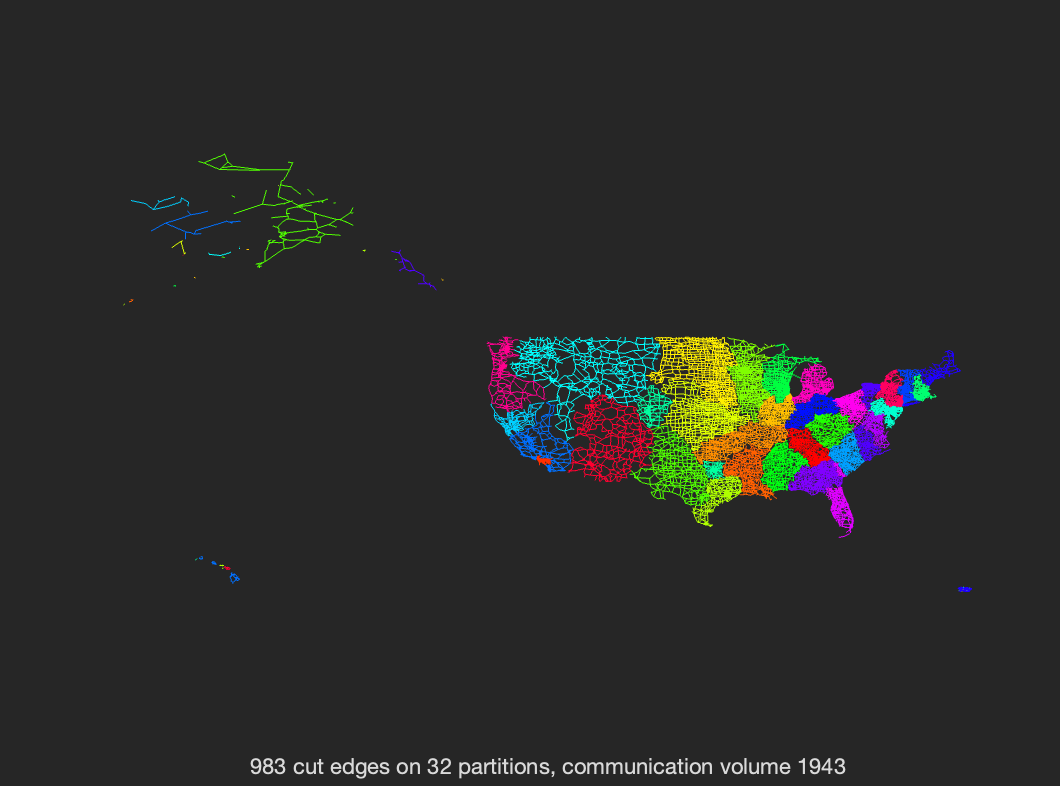
\includegraphics[width=\textwidth]{./media/usa_metis.png}
		\caption{USA with recursive bisection}
		\label{fig:usa_metis}
	\end{subfigure}%
	~
	\begin{subfigure}{0.5\textwidth}
		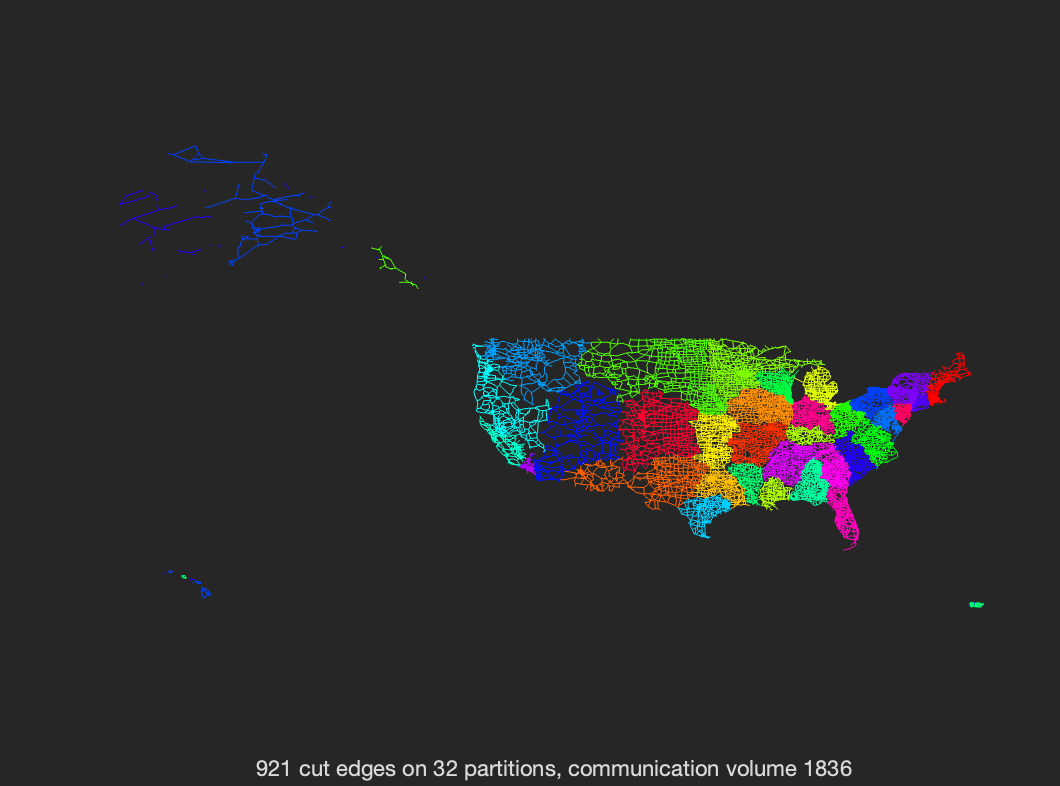
\includegraphics[width=\textwidth]{./media/usa_metis_k.png}
		\caption{USA with direct multiway partitioning}
		\label{fig:usa_metis_k}
	\end{subfigure}\\
	\begin{subfigure}{0.5\textwidth}
		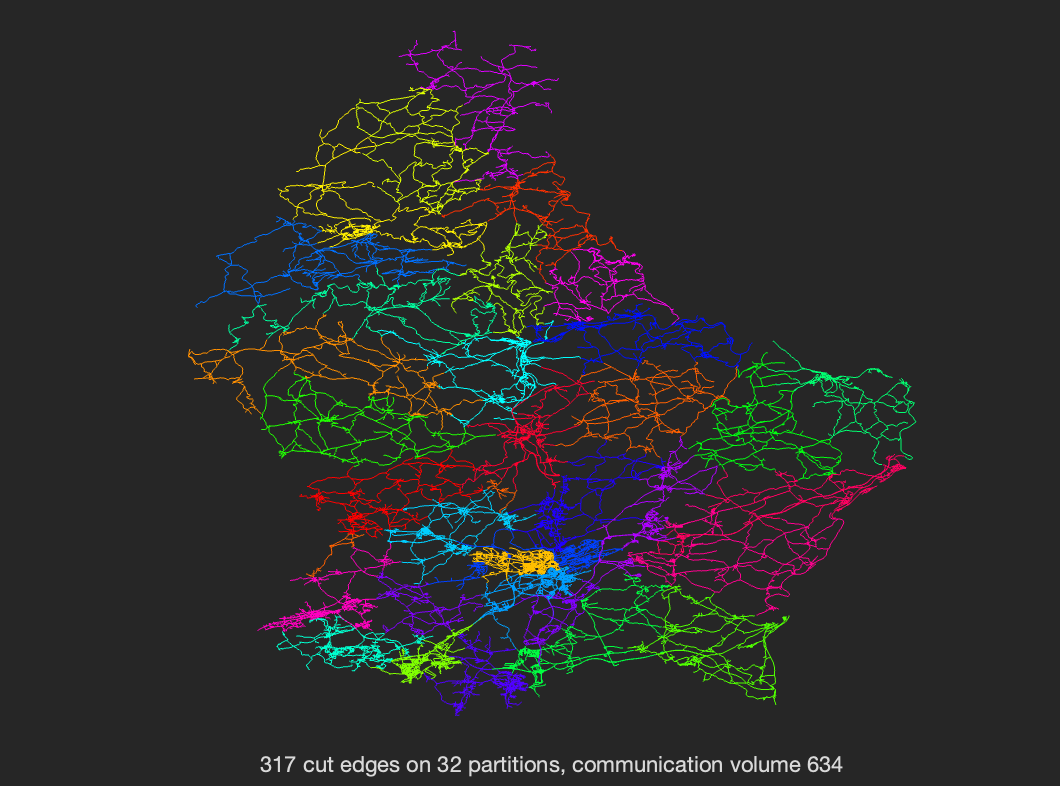
\includegraphics[width=\textwidth]{./media/lux_metis.png}
		\caption{Luxembourg with recursive bisection}
		\label{fig:lux_metis}
	\end{subfigure}%
	~
	\begin{subfigure}{0.5\textwidth}
		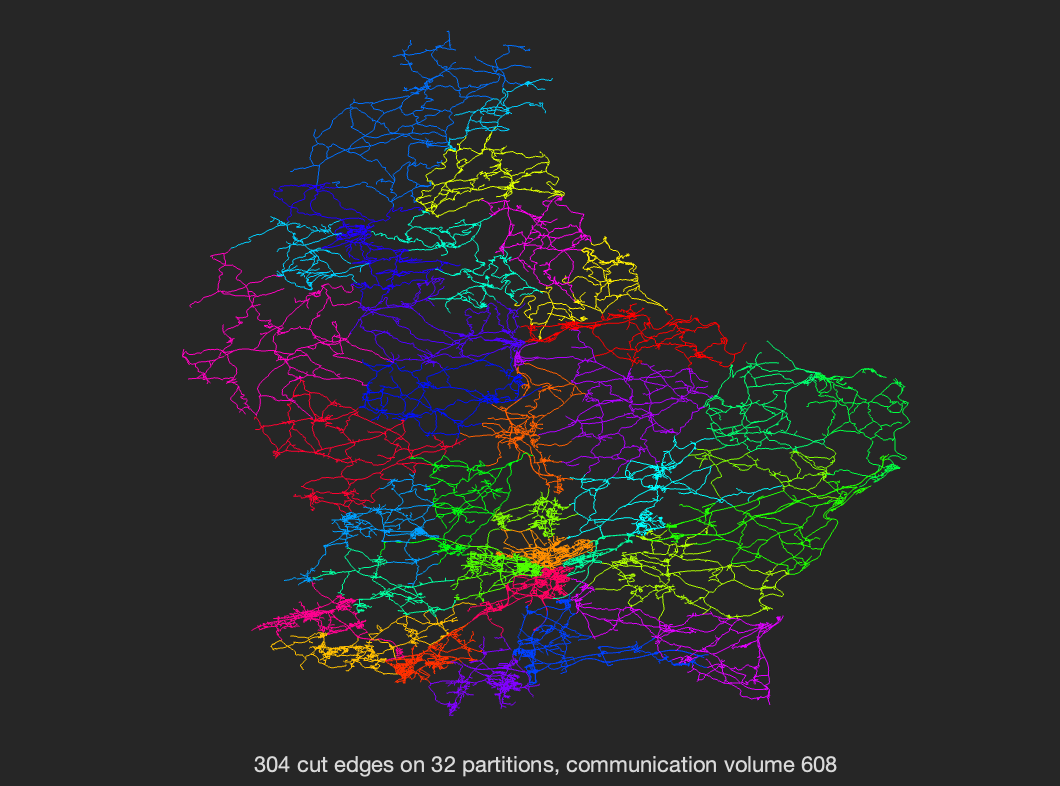
\includegraphics[width=\textwidth]{./media/lux_metis_k.png}
		\caption{Luxembourg with direct multiway partitioning}
		\label{fig:lux_metis_k}
	\end{subfigure}
	\begin{subfigure}{0.5\textwidth}
		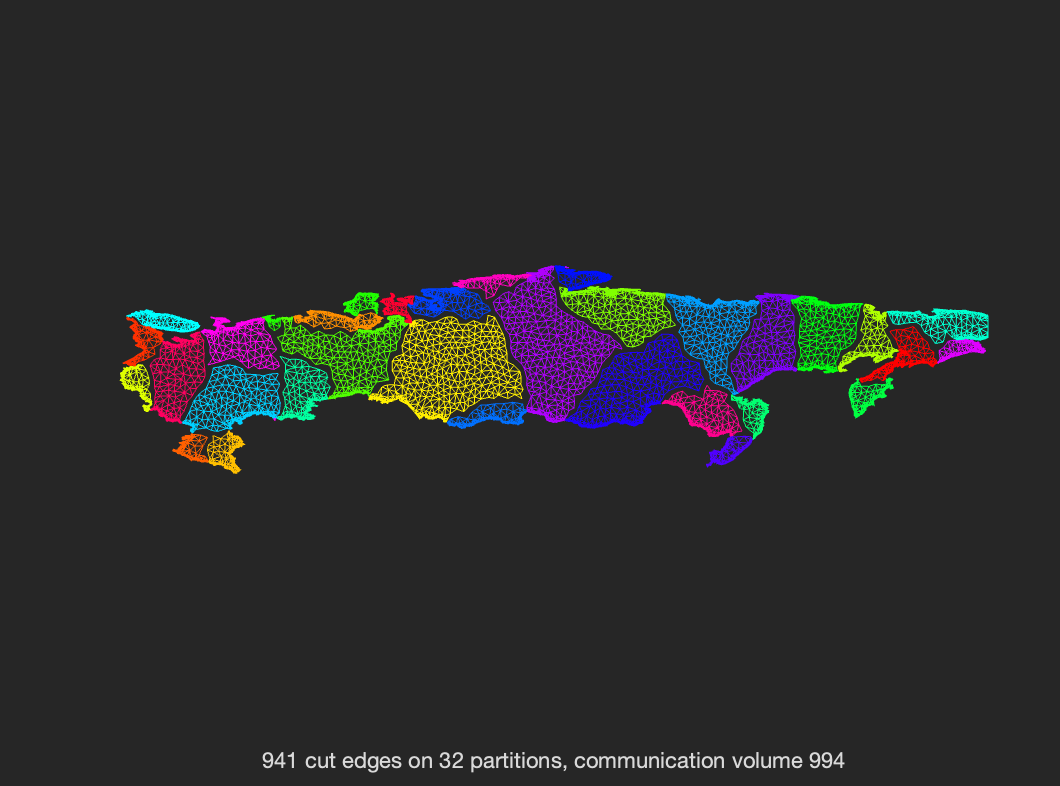
\includegraphics[width=\textwidth]{./media/ru_metis.png}
		\caption{Russia with recursive bisection}
		\label{fig:ru_metis}
	\end{subfigure}%
	~
	\begin{subfigure}{0.5\textwidth}
		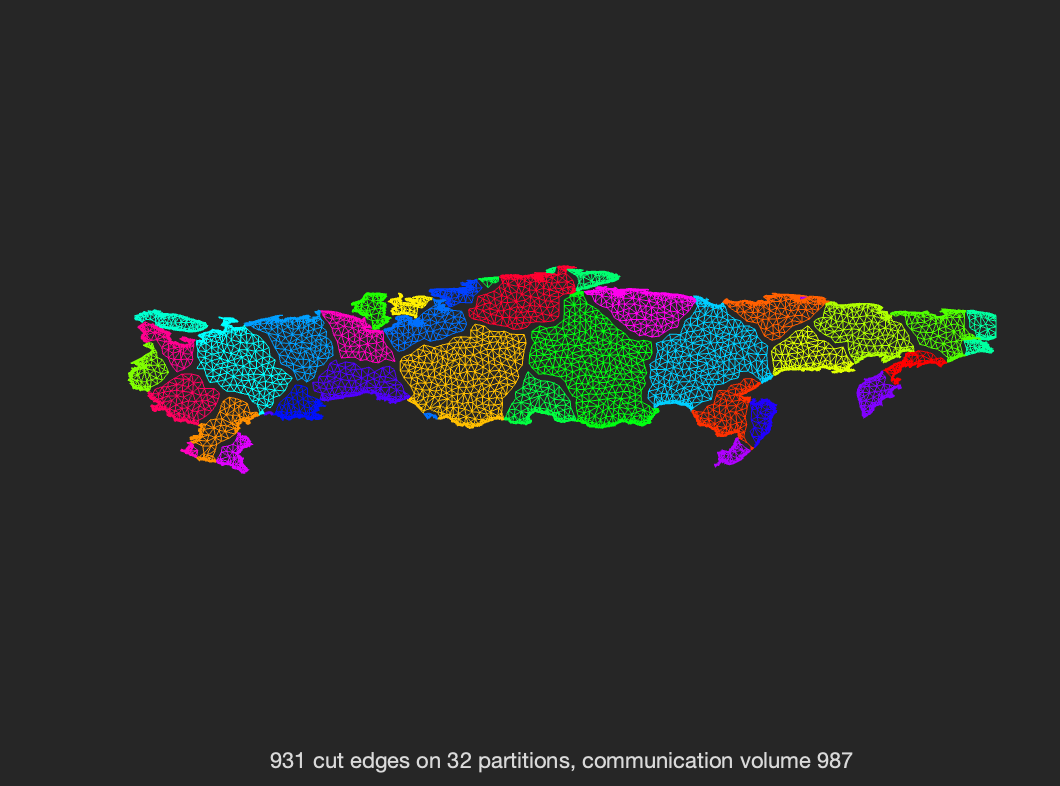
\includegraphics[width=\textwidth]{./media/ru_metis_k.png}
		\caption{Russia with direct multiway partitioning}
		\label{fig:ru_metis_k}
	\end{subfigure}

	\caption{Partitioning results for the graphs of USA, Luxemburg, and Russia
for 32 partitions}
	\label{fig:metis}
\end{figure}

